%!TEX root = ../../blob1.tex

\section{Comparing $n$-category definitions}
\label{sec:comparing-defs}

In \S\ref{sec:example:traditional-n-categories(fields)} we showed how to construct
a topological $n$-category from a traditional $n$-category; the morphisms of the 
topological $n$-category are string diagrams labeled by the traditional $n$-category.
In this appendix we sketch how to go the other direction, for $n=1$ and 2.
The basic recipe, given a topological $n$-category $\cC$, is to define the $k$-morphisms
of the corresponding traditional $n$-category to be $\cC(B^k)$, where
$B^k$ is the {\it standard} $k$-ball.
One must then show that the axioms of \S\ref{ss:n-cat-def} imply the traditional $n$-category axioms.
One should also show that composing the two arrows (between traditional and topological $n$-categories)
yields the appropriate sort of equivalence on each side.
Since we haven't given a definition for functors between topological $n$-categories
(the paper is already too long!), we do not pursue this here.

We emphasize that we are just sketching some of the main ideas in this appendix ---
it falls well short of proving the definitions are equivalent.

%\nn{cases to cover: (a) plain $n$-cats for $n=1,2$; (b) $n$-cat modules for $n=1$, also 2?;
%(c) $A_\infty$ 1-cat; (b) $A_\infty$ 1-cat module?; (e) tensor products?}

\subsection{$1$-categories over $\Set$ or $\Vect$}
\label{ssec:1-cats}
Given a topological $1$-category $\cX$ we construct a $1$-category in the conventional sense, $c(\cX)$.
This construction is quite straightforward, but we include the details for the sake of completeness, 
because it illustrates the role of structures (e.g. orientations, spin structures, etc) 
on the underlying manifolds, and 
to shed some light on the $n=2$ case, which we describe in \S \ref{ssec:2-cats}.

Let $B^k$ denote the \emph{standard} $k$-ball.
Let the objects of $c(\cX)$ be $c(\cX)^0 = \cX(B^0)$ and the morphisms of $c(\cX)$ be $c(\cX)^1 = \cX(B^1)$.
The boundary and restriction maps of $\cX$ give domain and range maps from $c(\cX)^1$ to $c(\cX)^0$.

Choose a homeomorphism $B^1\cup_{pt}B^1 \to B^1$.
Define composition in $c(\cX)$ to be the induced map $c(\cX)^1\times c(\cX)^1 \to c(\cX)^1$ 
(defined only when range and domain agree).
By isotopy invariance in $\cX$, any other choice of homeomorphism gives the same composition rule.
Also by isotopy invariance, composition is strictly associative.

Given $a\in c(\cX)^0$, define $\id_a \deq a\times B^1$.
By extended isotopy invariance in $\cX$, this has the expected properties of an identity morphism.


If the underlying manifolds for $\cX$ have further geometric structure, then we obtain certain functors.
The base case is for oriented manifolds, where we obtain no extra algebraic data.

For 1-categories based on unoriented manifolds, 
there is a map $*:c(\cX)^1\to c(\cX)^1$
coming from $\cX$ applied to an orientation-reversing homeomorphism (unique up to isotopy) 
from $B^1$ to itself.
Topological properties of this homeomorphism imply that 
$a^{**} = a$ (* is order 2), * reverses domain and range, and $(ab)^* = b^*a^*$
(* is an anti-automorphism).

For 1-categories based on Spin manifolds,
the the nontrivial spin homeomorphism from $B^1$ to itself which covers the identity
gives an order 2 automorphism of $c(\cX)^1$.

For 1-categories based on $\text{Pin}_-$ manifolds,
we have an order 4 antiautomorphism of $c(\cX)^1$.
For 1-categories based on $\text{Pin}_+$ manifolds,
we have an order 2 antiautomorphism and also an order 2 automorphism of $c(\cX)^1$,
and these two maps commute with each other.
%\nn{need to also consider automorphisms of $B^0$ / objects}

\noop{
\medskip

In the other direction, given a $1$-category $C$
(with objects $C^0$ and morphisms $C^1$) we will construct a topological
$1$-category $t(C)$.

If $X$ is a 0-ball (point), let $t(C)(X) \deq C^0$.
If $S$ is a 0-sphere, let $t(C)(S) \deq C^0\times C^0$.
If $X$ is a 1-ball, let $t(C)(X) \deq C^1$.
Homeomorphisms isotopic to the identity act trivially.
If $C$ has extra structure (e.g.\ it's a *-1-category), we use this structure
to define the action of homeomorphisms not isotopic to the identity
(and get, e.g., an unoriented topological 1-category).

The domain and range maps of $C$ determine the boundary and restriction maps of $t(C)$.

Gluing maps for $t(C)$ are determined by composition of morphisms in $C$.

For $X$ a 0-ball, $D$ a 1-ball and $a\in t(C)(X)$, define the product morphism 
$a\times D \deq \id_a$.
It is not hard to verify that this has the desired properties.

\medskip

The compositions of the constructions above, $$\cX\to c(\cX)\to t(c(\cX))$$ 
and $$C\to t(C)\to c(t(C)),$$ give back 
more or less exactly the same thing we started with.  

As we will see below, for $n>1$ the compositions yield a weaker sort of equivalence.
} %end \noop

\medskip

Similar arguments show that modules for topological 1-categories are essentially
the same thing as traditional modules for traditional 1-categories.


\subsection{Pivotal 2-categories}
\label{ssec:2-cats}
Let $\cC$ be a topological 2-category.
We will construct from $\cC$ a traditional pivotal 2-category.
(The ``pivotal" corresponds to our assumption of strong duality for $\cC$.)

We will try to describe the construction in such a way the the generalization to $n>2$ is clear,
though this will make the $n=2$ case a little more complicated than necessary.

Before proceeding, we must decide whether the 2-morphisms of our
pivotal 2-category are shaped like rectangles or bigons.
Each approach has advantages and disadvantages.
For better or worse, we choose bigons here.

Define the $k$-morphisms $C^k$ of $C$ to be $\cC(B^k)_E$, where $B^k$ denotes the standard
$k$-ball, which we also think of as the standard bihedron (a.k.a.\ globe).
(For $k=1$ this is an interval, and for $k=2$ it is a bigon.)
Since we are thinking of $B^k$ as a bihedron, we have a standard decomposition of the $\bd B^k$
into two copies of $B^{k-1}$ which intersect along the ``equator" $E \cong S^{k-2}$.
Recall that the subscript in $\cC(B^k)_E$ means that we consider the subset of $\cC(B^k)$
whose boundary is splittable along $E$.
This allows us to define the domain and range of morphisms of $C$ using
boundary and restriction maps of $\cC$.

Choosing a homeomorphism $B^1\cup B^1 \to B^1$ defines a composition map on $C^1$.
This is not associative, but we will see later that it is weakly associative.

Choosing a homeomorphism $B^2\cup B^2 \to B^2$ defines a ``vertical" composition map 
on $C^2$ (Figure \ref{fzo1}).
Isotopy invariance implies that this is associative.
We will define a ``horizontal" composition later.

\begin{figure}[t]
\begin{equation*}
\mathfig{.73}{tempkw/zo1}
\end{equation*}
\caption{Vertical composition of 2-morphisms}
\label{fzo1}
\end{figure}

Given $a\in C^1$, define $\id_a = a\times I \in C^2$ (pinched boundary).
Extended isotopy invariance for $\cC$ shows that this morphism is an identity for 
vertical composition.

Given $x\in C^0$, define $\id_x = x\times B^1 \in C^1$.
We will show that this 1-morphism is a weak identity.
This would be easier if our 2-morphisms were shaped like rectangles rather than bigons.

In showing that identity 1-morphisms have the desired properties, we will
rely heavily on the extended isotopy invariance of 2-morphisms in $\cC$.
This means we are free to add or delete product regions from 2-morphisms.

Let $a: y\to x$ be a 1-morphism.
Define 2-morphsims $a \to a\bullet \id_x$ and $a\bullet \id_x \to a$
as shown in Figure \ref{fzo2}.
\begin{figure}[t]
\begin{tikzpicture}
\newcommand{\rr}{6}
\newcommand{\vertex}{node[circle,fill=black,inner sep=1pt] {}}

\node(A) at (0,0) {
\begin{tikzpicture}
\node[red,left] at (0,0)  {$y$};
\draw (0,0) \vertex arc (-120:-105:\rr) node[red,below] {$a$} arc(-105:-90:\rr) \vertex node[red,below](x2) {$x$};
\draw (0,0) \vertex arc (120:105:\rr) node[red,above] {$a$} arc (105:90:\rr) \vertex node[red,above](x1) {$x$} -- (x2);
\begin{scope}
	\path[clip] (0,0) arc (-120:-60:\rr) arc (60:120:\rr);
	\foreach \x in {0,0.24,...,3} {
		\draw[green!50!brown] (\x,1) -- (\x,-1);
	}
\end{scope}
\draw[red, decorate,decoration={brace,amplitude=5pt}] ($(x1)+(0.2,-0.2)$) -- ($(x2)+(0.2,0.2)$) node[midway, xshift=0.7cm] {$x \times I$};
\end{tikzpicture}
};

\node(B) at (-4,-4) {
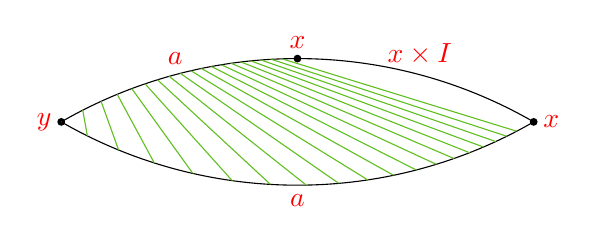
\begin{tikzpicture}
\node[red,left] at (0,0) {$y$};
\draw (0,0) \vertex 
	arc (120:105:\rr) node[red,above] {$a$}
	arc (105:90:\rr) node[red,above] {$x$} \vertex
	arc (90:75:\rr) node[red,above] {$x \times I$}
	arc (75:60:\rr) \vertex node[red,right] {$x$}
	arc (-60:-90:\rr) node[red,below] {$a$}
	arc (-90:-120:\rr);
\begin{scope}
	\path[clip] (0,0) arc (-120:-60:\rr) arc (60:120:\rr);
	\foreach \x in {0,0.48,...,9} {
		\draw[green!50!brown] (\x/4,1) -- (\x,-1);
	}
\end{scope}
\end{tikzpicture}
};

\node(C) at (4,-4) {
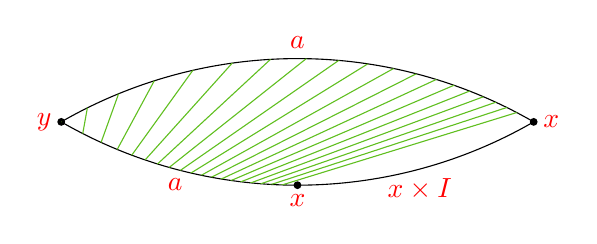
\begin{tikzpicture}[y=-1cm]
\node[red,left] at (0,0) {$y$};
\draw (0,0) \vertex 
	arc (120:105:\rr) node[red,below] {$a$}
	arc (105:90:\rr) node[red,below] {$x$} \vertex
	arc (90:75:\rr) node[red,below] {$x \times I$}
	arc (75:60:\rr) \vertex node[red,right] {$x$}
	arc (-60:-90:\rr) node[red,above] {$a$}
	arc (-90:-120:\rr);
\begin{scope}
	\path[clip] (0,0) arc (-120:-60:\rr) arc (60:120:\rr);
	\foreach \x in {0,0.48,...,9} {
		\draw[green!50!brown] (\x/4,1) -- (\x,-1);
	}
\end{scope}
\end{tikzpicture}
};

\draw[->] (A) -- (B);
\draw[->] (A) -- (C);
\end{tikzpicture}
\caption{Producing weak identities from half pinched products}
\label{fzo2}
\end{figure}
As suggested by the figure, these are two different reparameterizations
of a half-pinched version of $a\times I$.
We must show that the two compositions of these two maps give the identity 2-morphisms
on $a$ and $a\bullet \id_x$, as defined above.
Figure \ref{fzo3} shows one case.
\begin{figure}[t]
\begin{equation*}
\mathfig{.83}{tempkw/zo3}
\end{equation*}
\caption{Composition of weak identities, 1}
\label{fzo3}
\end{figure}
In the first step we have inserted a copy of $(x\times I)\times I$.
Figure \ref{fzo4} shows the other case.
\begin{figure}[t]
\begin{equation*}
\mathfig{.83}{tempkw/zo4}
\end{equation*}
\caption{Composition of weak identities, 2}
\label{fzo4}
\end{figure}
We identify a product region and remove it.

We define horizontal composition of 2-morphisms as shown in Figure \ref{fzo5}.
It is not hard to show that this is independent of the arbitrary (left/right) 
choice made in the definition, and that it is associative.
\begin{figure}[t]
\begin{equation*}
\mathfig{.83}{tempkw/zo5}
\end{equation*}
\caption{Horizontal composition of 2-morphisms}
\label{fzo5}
\end{figure}

%\nn{need to find a list of axioms for pivotal 2-cats to check}


\subsection{$A_\infty$ $1$-categories}
\label{sec:comparing-A-infty}
In this section, we make contact between the usual definition of an $A_\infty$ category 
and our definition of a topological $A_\infty$ $1$-category, from \S \ref{ss:n-cat-def}.

\medskip

Given a topological $A_\infty$ $1$-category $\cC$, we define an ``$m_k$-style" 
$A_\infty$ $1$-category $A$ as follows.
The objects of $A$ are $\cC(pt)$.
The morphisms of $A$, from $x$ to $y$, are $\cC(I; x, y)$
($\cC$ applied to the standard interval with boundary labeled by $x$ and $y$).
For simplicity we will now assume there is only one object and suppress it from the notation.

A choice of homeomorphism $I\cup I \to I$ induces a chain map $m_2: A\times A\to A$.
We now have two different homeomorphisms $I\cup I\cup I \to I$, but they are isotopic.
Choose a specific 1-parameter family of homeomorphisms connecting them; this induces
a degree 1 chain homotopy $m_3:A\ot A\ot A\to A$.
Proceeding in this way we define the rest of the $m_i$'s.
It is straightforward to verify that they satisfy the necessary identities.

\medskip

In the other direction, we start with an alternative conventional definition of an $A_\infty$ algebra:
an algebra $A$ for the $A_\infty$ operad.
(For simplicity, we are assuming our $A_\infty$ 1-category has only one object.)
We are free to choose any operad with contractible spaces, so we choose the operad
whose $k$-th space is the space of decompositions of the standard interval $I$ into $k$
parameterized copies of $I$.
Note in particular that when $k=1$ this implies a $C_*(\Homeo(I))$ action on $A$.
(Compare with Example \ref{ex:e-n-alg} and the discussion which precedes it.)
Given a non-standard interval $J$, we define $\cC(J)$ to be
$(\Homeo(I\to J) \times A)/\Homeo(I\to I)$,
where $\beta \in \Homeo(I\to I)$ acts via $(f, a) \mapsto (f\circ \beta\inv, \beta_*(a))$.
\nn{check this}
Note that $\cC(J) \cong A$ (non-canonically) for all intervals $J$.
We define a $\Homeo(J)$ action on $\cC(J)$ via $g_*(f, a) = (g\circ f, a)$.
The $C_*(\Homeo(J))$ action is defined similarly.

Let $J_1$ and $J_2$ be intervals.
We must define a map $\cC(J_1)\ot\cC(J_2)\to\cC(J_1\cup J_2)$.
Choose a homeomorphism $g:I\to J_1\cup J_2$.
Let $(f_i, a_i)\in \cC(J_i)$.
We have a parameterized decomposition of $I$ into two intervals given by
$g\inv \circ f_i$, $i=1,2$.
Corresponding to this decomposition the operad action gives a map $\mu: A\ot A\to A$.
Define the gluing map to send $(f_1, a_1)\ot (f_2, a_2)$ to $(g, \mu(a_1\ot a_2))$.
Operad associativity for $A$ implies that this gluing map is independent of the choice of
$g$ and the choice of representative $(f_i, a_i)$.

It is straightforward to verify the remaining axioms for a topological $A_\infty$ 1-category.







\noop { %%%%%%%%%%%%%%%%%%%%%%%%%%%%%%%%%%

That definition associates a chain complex to every interval, and we begin by giving an alternative definition that is entirely in terms of the chain complex associated to the standard interval $[0,1]$. 
\begin{defn}
A \emph{topological $A_\infty$ category on $[0,1]$} $\cC$ has a set of objects $\Obj(\cC)$, 
and for each $a,b \in \Obj(\cC)$, a chain complex $\cC_{a,b}$, along with
\begin{itemize}
\item an action of the operad of $\Obj(\cC)$-labeled cell decompositions
\item and a compatible action of $\CD{[0,1]}$.
\end{itemize}
\end{defn}
Here the operad of cell decompositions of $[0,1]$ has operations indexed by a finite set of 
points $0 < x_1< \cdots < x_k < 1$, cutting $[0,1]$ into subintervals.
An $X$-labeled cell decomposition labels $\{0, x_1, \ldots, x_k, 1\}$ by $X$.
Given two cell decompositions $\cJ^{(1)}$ and $\cJ^{(2)}$, and an index $m$, we can compose 
them to form a new cell decomposition $\cJ^{(1)} \circ_m \cJ^{(2)}$ by inserting the points 
of $\cJ^{(2)}$ linearly into the $m$-th interval of $\cJ^{(1)}$.
In the $X$-labeled case, we insist that the appropriate labels match up.
Saying we have an action of this operad means that for each labeled cell decomposition 
$0 < x_1< \cdots < x_k < 1$, $a_0, \ldots, a_{k+1} \subset \Obj(\cC)$, there is a chain 
map $$\cC_{a_0,a_1} \tensor \cdots \tensor \cC_{a_k,a_{k+1}} \to \cC_{a_0,a_{k+1}}$$ and these 
chain maps compose exactly as the cell decompositions.
An action of $\CD{[0,1]}$ is compatible with an action of the cell decomposition operad 
if given a decomposition $\pi$, and a family of diffeomorphisms $f \in \CD{[0,1]}$ which 
is supported on the subintervals determined by $\pi$, then the two possible operations 
(glue intervals together, then apply the diffeomorphisms, or apply the diffeormorphisms 
separately to the subintervals, then glue) commute (as usual, up to a weakly unique homotopy).

Translating between this notion and the usual definition of an $A_\infty$ category is now straightforward.
To restrict to the standard interval, define $\cC_{a,b} = \cC([0,1];a,b)$.
Given a cell decomposition $0 < x_1< \cdots < x_k < 1$, we use the map (suppressing labels)
$$\cC([0,1])^{\tensor k+1} \to \cC([0,x_1]) \tensor \cdots \tensor \cC[x_k,1] \to \cC([0,1])$$
where the factors of the first map are induced by the linear isometries $[0,1] \to [x_i, x_{i+1}]$, and the second map is just gluing.
The action of $\CD{[0,1]}$ carries across, and is automatically compatible.
Going the other way, we just declare $\cC(J;a,b) = \cC_{a,b}$, pick a diffeomorphism 
$\phi_J : J \isoto [0,1]$ for every interval $J$, define the gluing map 
$\cC(J_1) \tensor \cC(J_2) \to \cC(J_1 \cup J_2)$ by the first applying 
the cell decomposition map for $0 < \frac{1}{2} < 1$, then the self-diffeomorphism of $[0,1]$ 
given by $\frac{1}{2} (\phi_{J_1} \cup (1+ \phi_{J_2})) \circ \phi_{J_1 \cup J_2}^{-1}$.
You can readily check that this gluing map is associative on the nose. \todo{really?}

%First recall the \emph{coloured little intervals operad}. Given a set of labels $\cL$, the operations are indexed by \emph{decompositions of the interval}, each of which is a collection of disjoint subintervals $\{(a_i,b_i)\}_{i=1}^k$ of $[0,1]$, along with a labeling of the complementary regions by $\cL$, $\{l_0, \ldots, l_k\}$.  Given two decompositions $\cJ^{(1)}$ and $\cJ^{(2)}$, and an index $m$ such that $l^{(1)}_{m-1} = l^{(2)}_0$ and $l^{(1)}_{m} = l^{(2)}_{k^{(2)}}$, we can form a new decomposition by inserting the intervals of $\cJ^{(2)}$ linearly inside the $m$-th interval of $\cJ^{(1)}$. We call the resulting decomposition $\cJ^{(1)} \circ_m \cJ^{(2)}$.

%\begin{defn}
%A \emph{topological $A_\infty$ category} $\cC$ has a set of objects $\Obj(\cC)$ and for each $a,b \in \Obj(\cC)$ a chain complex $\cC_{a,b}$, along with a compatible `composition map' and an `action of families of diffeomorphisms'.

%A \emph{composition map} $f$ is a family of chain maps, one for each decomposition of the interval, $f_\cJ : A^{\tensor k} \to A$, making $\cC$ into a category over the coloured little intervals operad, with labels $\cL = \Obj(\cC)$. Thus the chain maps satisfy the identity 
%\begin{equation*}
%f_{\cJ^{(1)} \circ_m \cJ^{(2)}} = f_{\cJ^{(1)}} \circ (\id^{\tensor m-1} \tensor f_{\cJ^{(2)}} \tensor \id^{\tensor k^{(1)} - m}).
%\end{equation*}

%An \emph{action of families of diffeomorphisms} is a chain map $ev: \CD{[0,1]} \tensor A \to A$, such that 
%\begin{enumerate}
%\item The diagram 
%\begin{equation*}
%\xymatrix{
%\CD{[0,1]} \tensor \CD{[0,1]} \tensor A \ar[r]^{\id \tensor ev} \ar[d]^{\circ \tensor \id} & \CD{[0,1]} \tensor A \ar[d]^{ev} \\
%\CD{[0,1]} \tensor A \ar[r]^{ev} & A
%}
%\end{equation*}
%commutes up to weakly unique homotopy.
%\item If $\phi \in \Diff([0,1])$ and $\cJ$ is a decomposition of the interval, we obtain a new decomposition $\phi(\cJ)$ and a collection $\phi_m \in \Diff([0,1])$ of diffeomorphisms obtained by taking the restrictions $\restrict{\phi}{[a_m,b_m]} : [a_m,b_m] \to [\phi(a_m),\phi(b_m)]$ and pre- and post-composing these with the linear diffeomorphisms $[0,1] \to [a_m,b_m]$ and $[\phi(a_m),\phi(b_m)] \to [0,1]$. We require that
%\begin{equation*}
%\phi(f_\cJ(a_1, \cdots, a_k)) = f_{\phi(\cJ)}(\phi_1(a_1), \cdots, \phi_k(a_k)).
%\end{equation*}
%\end{enumerate}
%\end{defn}

From a topological $A_\infty$ category on $[0,1]$ $\cC$ we can produce a `conventional' 
$A_\infty$ category $(A, \{m_k\})$ as defined in, for example, \cite{MR1854636}.
We'll just describe the algebra case (that is, a category with only one object), 
as the modifications required to deal with multiple objects are trivial.
Define $A = \cC$ as a chain complex (so $m_1 = d$).
Define $m_2 : A\tensor A \to A$ by $f_{\{(0,\frac{1}{2}),(\frac{1}{2},1)\}}$.
To define $m_3$, we begin by taking the one parameter family $\phi_3$ of diffeomorphisms 
of $[0,1]$ that interpolates linearly between the identity and the piecewise linear 
diffeomorphism taking $\frac{1}{4}$ to $\frac{1}{2}$ and $\frac{1}{2}$ to $\frac{3}{4}$, and then define
\begin{equation*}
m_3(a,b,c) = ev(\phi_3, m_2(m_2(a,b), c)).
\end{equation*}

It's then easy to calculate that
\begin{align*}
d(m_3(a,b,c)) & = ev(d \phi_3, m_2(m_2(a,b),c)) - ev(\phi_3 d m_2(m_2(a,b), c)) \\
 & = ev( \phi_3(1), m_2(m_2(a,b),c)) - ev(\phi_3(0), m_2 (m_2(a,b),c)) - \\ & \qquad - ev(\phi_3, m_2(m_2(da, b), c) + (-1)^{\deg a} m_2(m_2(a, db), c) + \\ & \qquad \quad + (-1)^{\deg a+\deg b} m_2(m_2(a, b), dc) \\
 & = m_2(a , m_2(b,c)) - m_2(m_2(a,b),c) - \\ & \qquad - m_3(da,b,c) + (-1)^{\deg a + 1} m_3(a,db,c) + \\ & \qquad \quad + (-1)^{\deg a + \deg b + 1} m_3(a,b,dc), \\
\intertext{and thus that}
m_1 \circ m_3 & =  m_2 \circ (\id \tensor m_2) - m_2 \circ (m_2 \tensor \id) - \\ & \qquad - m_3 \circ (m_1 \tensor \id \tensor \id) - m_3 \circ (\id \tensor m_1 \tensor \id) - m_3 \circ (\id \tensor \id \tensor m_1)
\end{align*}
as required (c.f. \cite[p. 6]{MR1854636}).
\todo{then the general case.}
We won't describe a reverse construction (producing a topological $A_\infty$ category 
from a ``conventional" $A_\infty$ category), but we presume that this will be easy for the experts.

} %%%%% end \noop %%%%%%%%%%%%%%%%%%%%%%%%%%%%%%%%%